\documentclass{standalone}

\usepackage[english]{babel}
\usepackage[linesnumbered, ruled, vlined]{algorithm2e}

\usepackage{caption}
\usepackage{amsmath,amssymb}
\usepackage[dvipsnames]{xcolor}

% to create listings

\usepackage{listings, lstautogobble}
\lstset{
  autogobble=true,
  frame=single,
}

\lstdefinelanguage{coq}[Objective]{Caml}{
  morekeywords={Structure, Definition, Inductive, list, return},
  sensitive=true
}

% to define font size

\usepackage{ulem}
\usepackage{moresize}
\usepackage{anyfontsize}

% to use tikz and its libraries

\usepackage{tikz-timing}
\usepackage{tikz}

\usetikzlibrary{backgrounds}
\usetikzlibrary{positioning, calc, arrows, shapes, automata, petri, patterns}

% to use tikzmark, to place and refer to marks outside the current figure

\tikzset{every picture/.style={remember picture}}

% styles for transitions

\tikzset{transition/.append style={fill=black!20, thick}}
\tikzset{transition/.append style={fill=black!20, thick}}

% styles for test and inhib arcs.

\tikzstyle{test}=[pre, *-]
\tikzstyle{inhib}=[pre, o-]

% to use colors

\usepackage{xcolor}

%%%%%%%%%%%%%%%%%%%%%%%%%%%%%%%%%%%%%%%%%%%%%%%%%%
%                  BEGIN DOCUMENT                %
%%%%%%%%%%%%%%%%%%%%%%%%%%%%%%%%%%%%%%%%%%%%%%%%%%

\begin{document}

\begin{tikzpicture}

  \node[] (pn-start) {
    \begin{tikzpicture}
      \node[place, tokens=3] (p0) [label={above:$p$}] {};
      
      \node[transition] (t0) [below left=.5cm of p0, label={left:
        \begin{tabular}{@{}c@{}}
          $t_0$ \\
          $[2,\infty]$ \\
          \textcolor{Green}{${<}2{>}$}\\
        \end{tabular}
      }] {} edge[pre, bend left] (p0);
      
      \node[transition] (t1) [below right=.5cm of p0, label={right:
        \begin{tabular}{@{}c@{}}
          $t_1$ \\
          $[2,\infty]$ \\
          \textcolor{Green}{${<}2{>}$}\\
        \end{tabular}}] {}
      edge[pre, bend right] (p0);

      \draw (t0.south) edge[->,dotted, bend right=45] (t1.south);

    \end{tikzpicture}
  };

  \node[] (pn-re) at ($(pn-start)+(6,0)$){
    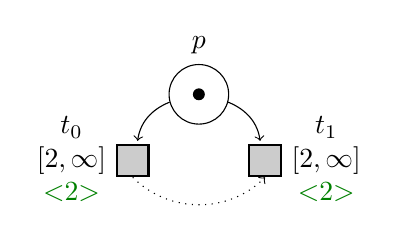
\begin{tikzpicture}
      \node[place, tokens=1] (p0) [label={above:$p$}] {};
      
      \node[transition] (t0) [below left=.5cm of p0, label={left:
        \begin{tabular}{@{}c@{}}
          $t_0$ \\
          $[2,\infty]$ \\
          \textcolor{Green}{${<}2{>}$}\\
        \end{tabular}
      }] {} edge[pre, bend left] (p0);
      
      \node[transition] (t1) [below right=.5cm of p0, label={right:
        \begin{tabular}{@{}c@{}}
          $t_1$ \\
          $[2,\infty]$ \\
          \textcolor{Green}{${<}2{>}$}\\
        \end{tabular}}] {}
      edge[pre, bend right] (p0);

      \draw (t0.south) edge[->,dotted, bend right=45] (t1.south);

    \end{tikzpicture}
  };

  \node[] (pn-fe) at ($(pn-re)+(6,0)$){
    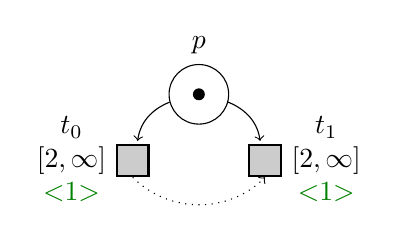
\begin{tikzpicture}
      \node[place, tokens=1] (p0) [label={above:$p$}] {};
      
      \node[transition] (t0) [below left=.5cm of p0, label={left:
        \begin{tabular}{@{}c@{}}
          $t_0$ \\
          $[2,\infty]$ \\
          \textcolor{Green}{${<}1{>}$}\\
        \end{tabular}
      }] {} edge[pre, bend left] (p0);
      
      \node[transition] (t1) [below right=.5cm of p0, label={right:
        \begin{tabular}{@{}c@{}}
          $t_1$ \\
          $[2,\infty]$ \\
          \textcolor{Green}{${<}1{>}$}\\
        \end{tabular}}] {}
      edge[pre, bend right] (p0);

      \draw (t0.south) edge[->,dotted, bend right=45] (t1.south);

    \end{tikzpicture}
  };

  \node at ($(pn-start)!.5!(pn-re)$) {\huge $\xrightarrow{\uparrow}$};
  \node at ($(pn-re)!.5!(pn-fe)$) {\huge $\xrightarrow{\downarrow}$};

  % VHDL
  
  \node[anchor=north,] (legend-start) at ($(pn-start.south)-(3,0)$) {
    \begin{tabular}{@{}|l|@{}}
      \hline
      \multicolumn{1}{@{}|c|@{}}{PCI $id_p$} \\
      \hline
      $\mathtt{s\_marking}=3$ \\
      $\mathtt{pauths}$ to $id_{t_0}=\mathtt{true}$ \\
      $\mathtt{pauths}$ to $id_{t_1}=\mathtt{true}$ \\
      \hline
      \multicolumn{1}{@{}|c|@{}}{TCI $id_{t_0}$} \\
      \hline
      $\mathtt{pauths}$ from $id_p=\mathtt{true}$ \\
      \textcolor{Green}{$\mathtt{s\_time\_counter}=2$} \\
      $\mathtt{fired}=\mathtt{true}$ \\
      \hline
      \multicolumn{1}{@{}|c|@{}}{TCI $id_{t_1}$} \\
      \hline
      $\mathtt{pauths}$ from $id_p=\mathtt{true}$ \\
      \textcolor{Green}{$\mathtt{s\_time\_counter}=2$} \\
      $\mathtt{fired}=\mathtt{true}$ \\
      \hline
    \end{tabular}
  };

  \node[anchor=north,] (legend-re) at ($(pn-start.south)!.5!(pn-re.south)$) {
    \begin{tabular}{@{}|l|@{}}
      \hline
      \multicolumn{1}{@{}|c|@{}}{PCI $id_p$} \\
      \hline
      $\mathtt{s\_marking}=1$ \\
      $\mathtt{pauths}$ to $id_{t_0}=\mathtt{true}$ \\
      $\mathtt{pauths}$ to $id_{t_1}=\mathtt{true}$ \\
      \hline
      \multicolumn{1}{@{}|c|@{}}{TCI $id_{t_0}$} \\
      \hline
      $\mathtt{pauths}$ from $id_p=\mathtt{true}$ \\
      \textcolor{Green}{$\mathtt{s\_time\_counter}=2$} \\
      $\mathtt{fired}=\mathtt{true}$ \\
      \hline
      \multicolumn{1}{@{}|c|@{}}{TCI $id_{t_1}$} \\
      \hline
      $\mathtt{pauths}$ from $id_p=\mathtt{true}$ \\
      \textcolor{Green}{$\mathtt{s\_time\_counter}=2$} \\
      $\mathtt{fired}=\mathtt{true}$ \\
      \hline
    \end{tabular}
  };

  \node[anchor=north,] (legend-re-stab) at ($(pn-re.south)!.5!(pn-fe.south)$) {
    \begin{tabular}{@{}|l|@{}}
      \hline
      \multicolumn{1}{@{}|c|@{}}{PCI $id_p$} \\
      \hline
      $\mathtt{s\_marking}=1$ \\
      $\mathtt{pauths}$ to $id_{t_0}=\mathtt{true}$ \\
      \textcolor{red}{$\mathtt{pauths}$ to $id_{t_1}=\mathtt{false}$} \\
      \hline
      \multicolumn{1}{@{}|c|@{}}{TCI $id_{t_0}$} \\
      \hline
      $\mathtt{pauths}$ from $id_p=\mathtt{true}$ \\
      \textcolor{Green}{$\mathtt{s\_time\_counter}=2$} \\
      $\mathtt{fired}=\mathtt{true}$ \\
      \hline
      \multicolumn{1}{@{}|c|@{}}{TCI $id_{t_1}$} \\
      \hline
      \textcolor{red}{$\mathtt{pauths}$ from $id_p=\mathtt{false}$} \\
      \textcolor{Green}{$\mathtt{s\_time\_counter}=2$} \\
      \textcolor{red}{$\mathtt{fired}=\mathtt{false}$} \\
      \hline
    \end{tabular}
  };

  \node[anchor=north,] (legend-fe) at ($(pn-fe.south)+(3,0)$) {
    \begin{tabular}{@{}|l|@{}}
      \hline
      \multicolumn{1}{@{}|c|@{}}{PCI $id_p$} \\
      \hline
      $\mathtt{s\_marking}=1$ \\
      $\mathtt{pauths}$ to $id_{t_0}=\mathtt{true}$ \\
      $\mathtt{pauths}$ to $id_{t_1}=\mathtt{false}$ \\
      \hline
      \multicolumn{1}{@{}|c|@{}}{TCI $id_{t_0}$} \\
      \hline
      $\mathtt{pauths}$ from $id_p=\mathtt{true}$ \\
      \textcolor{Green}{$\mathtt{s\_time\_counter}=1$} \\
      $\mathtt{fired}=\mathtt{true}$ \\
      \hline
      \multicolumn{1}{@{}|c|@{}}{TCI $id_{t_1}$} \\
      \hline
      $\mathtt{pauths}$ from $id_p=\mathtt{false}$ \\
      \textcolor{red}{$\mathtt{s\_time\_counter}=3$} \\
      $\mathtt{fired}=\mathtt{false}$ \\
      \hline
    \end{tabular}
  };

  \node at ($(legend-start)!.5!(legend-re)$) {\huge $\xrightarrow{\uparrow}$};
  \node at ($(legend-re)!.5!(legend-re-stab)$) {\huge $\xrightarrow{\rightsquigarrow}$};
  \node at ($(legend-re-stab)!.5!(legend-fe)$) {\huge $\xrightarrow{\downarrow}$};
  
\end{tikzpicture}

\end{document}
%%% Local Variables:
%%% mode: latex
%%% TeX-master: t
%%% End:
